\subsection{Half-precision floating-point numbers}
\label{sec:half2}
A significant performance improvement was achieved by transitioning from single-precision floating-point numbers to half-precision floating-point numbers.
Half-precision floating-point numbers are 16-bit floating-point numbers with 11 bits of significand precision, which is enough for the 10-bit pixel values.
The utilization of half precision floating-point numbers yield notable gains due the dedicated hardware present in the \gls{alu} on the \gls{volta} \gls{gpu} \cite{CUDA2023}.
\footnote{This should not be confused with Tensor cores, which also operate on half-precision floating-point numbers but are not employed in this project}.
This dedicated hardware allows for \gls{simd} operations on a specialized data format called \gls{half2} that stores two half precision floats, almost doubleing throughput \cite{nvidiaHalf2ArithmeticFunctions2023}\cite{hoExploitingHalfPrecision2017}.

The use of \gls{half2} is particularly useful in this context, as each row costist of alternating polarization channels.
This means that the incoming data can be cast directly to \gls{half2} during the unpacking phase, as follows:



\begin{figure}[H]
    \centering
    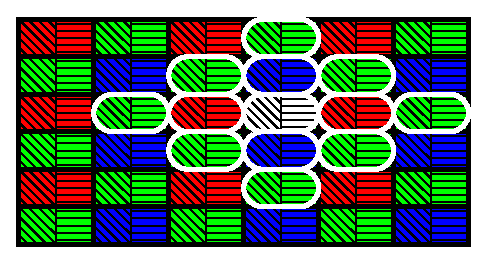
\includegraphics[width=0.45\textwidth]{figures/polarized_image/half2_conv.pdf}
    \caption{Vusialization of the convolution performed on the \gls{half2} data type. The pairs of pixels encircled are stored in a single \gls{half2} variable.}
    \label{fig:half2_conv}
\end{figure}

A disadvantage of using \gls{half2} is that every arithmetic operation, like multiplication, has to be performed using spceial function calls \cite{nvidiaHalf2ArithmeticFunctions2023}.
To solve this the code generator, discussed in Section \todo, was modified to generate the correct function calls as shown in Listing \ref{listing:generated_function}.

\subsubsection{Small Infinity Bug}
Half-precision floating points consider any value exceeding $65504$ as infinity \cite{HalfprecisionFloatingpointFormat2023}.
This can pose a problem when performing calculations that might exceed this threshold during intermediate steps, resulting in the value being treated as infinity.
In the preprocessing phase, this issue occasionally arises since the \code{P010_10LE} format utilizes the 10 most significant bits of a 16-bit integer, approaching the limit of half-precision floating points.

This was particularly problematic when the resulting values were cast to integers, as the resulting value would be zero, causing unexpected black spots in the image.
To mitigate this problem, the floating-point values are now cast to integers within the range of 0 to 1023, followed by a left bitshift of 6 bits to conform to the \code{P010_10LE} format.


